% =====================================================================
\chapter{Related Work}
\label{ch:related}
% =====================================================================

This chapter reviews the literature on hallucination detection and locates the present
dissertation within it. We group the field into four families, sketched in
Figure~\ref{fig:taxonomy}, and devote the most attention to the internal-state family
that this work extends. The chapter closes by describing the benchmarks the area uses,
the open problems it has identified, and the specific slot this dissertation occupies.

\begin{figure}[t]
\centering
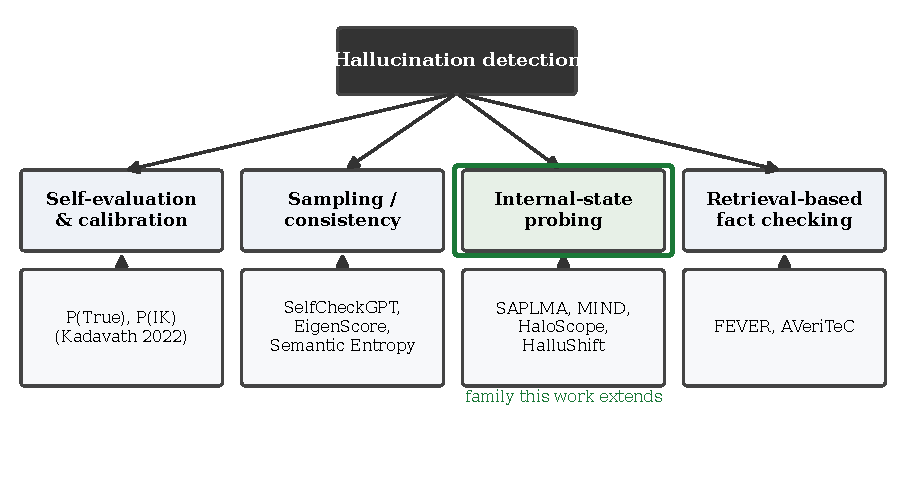
\includegraphics[width=0.96\textwidth]{images/ch03_related_work/ch03_1_taxonomy.pdf}
\caption{Four families of hallucination detection. This dissertation works in the
internal-state probing family (outlined), which reads a model's own activations and is
the cheapest to run at inference time.}
\label{fig:taxonomy}
\end{figure}

\section{Why surface-overlap metrics are not enough}

The earliest way to judge a generation was to compare it, word for word, against a
reference using overlap scores such as ROUGE or BLEU. These remain common as headline
numbers, but they measure surface similarity, not truth. The standard cautionary example
makes the point: the sentence ``Paris is the capital of Germany'' shares almost every
word with ``Paris is the capital of France'' and would earn a near-perfect overlap
score, despite being false. Surface form is a poor proxy for meaning, and a worse proxy
for factual correctness. The field has therefore moved to \emph{semantic} detectors that
do not rely on word overlap, and these fall into the four families below.

\section{Family I: self-evaluation and calibration}

The first idea is to ask the model to judge itself. The line begins with work showing
that large models are often reasonably \emph{calibrated}: the probability they assign to
an answer tracks how often that answer is correct~\cite{kadavath2022know}. Two probes
from that work are still influential. The first reads the probability the model assigns
to the token ``True'' after being asked to evaluate its own answer; the second trains a
small head to predict, from the question alone, whether the model is likely to answer
correctly. Both establish that a usable uncertainty signal exists inside the model, and
both are ancestors of the probing classifiers discussed later. Their limitation is that
self-evaluation tends to generalise only partially: a probe tuned on one task degrades
under distribution shift, a recurring theme that returns in our own transfer results.

\section{Family II: sampling and consistency}

A second family ignores the internals entirely and treats the model as a black box. The
idea is simple: generate an answer, then draw several more samples at a higher
temperature, and check whether they agree. Factual content tends to stay stable across
samples, while fabricated content tends to wobble. The canonical method,
SelfCheckGPT~\cite{manakul2023selfcheckgpt}, implements this consistency check at several
levels of abstraction, from word-overlap to a natural-language-inference model
(abbreviated NLI: a classifier that decides whether one sentence entails or contradicts
another). On a benchmark of generated biographies it detects non-factual sentences well
and needs no labels, no internals, and no retrieval --- only the ability to sample.

The weakness of this family is cost. Drawing roughly twenty extra generations per answer
makes detection many times more expensive than the original generation, which is exactly
the gap that motivates internal-state methods. Related sampling-based methods include
semantic entropy, which clusters samples that mean the same thing and measures the
entropy over those clusters~\cite{kuhn2023semantic}, and an embedding-space method,
EigenScore, which inspects the eigenvalues of the covariance of several sampled
generations to gauge how semantically spread out they are~\cite{chen2024inside}; here
EigenScore is the scoring rule from the INSIDE method, which we later use as a baseline.
These methods are accurate but inherit the sampling cost, and semantic entropy
additionally needs an auxiliary NLI model loaded alongside the generator.

\section{Family III: internal-state probing}
\label{sec:internal}

The third family --- the one this dissertation extends --- asks whether truth is written
into the activations themselves. If it is, a detector can read it from a single forward
pass, with no sampling and no retrieval.

\subsection{SAPLMA: hidden states reveal untruths}

The family is usually traced to the finding that a model's hidden states ``know'' when
the model is producing a falsehood, even when the surface output gives no
sign~\cite{azaria2023saplma}. That work, SAPLMA, hand-built a corpus of true and false
statements, fed each statement to the model, and trained a small feed-forward classifier
on the activations the model produced while reading it. A mid-network layer carried the
strongest signal, and the probe clearly beat surface-probability baselines, confirming
that the relevant information lives in the hidden state rather than in the output logits.
The two limitations of this work --- its labels were produced by hand, which caps the
data scale, and its statements were \emph{read} rather than \emph{generated} by the model
--- set the agenda for what followed.

\subsection{MIND: automatic labels and real-time detection}

The method this dissertation builds on, MIND~\cite{su2024mind}, removes the hand-labelling
bottleneck. It generates its own training data from encyclopedia text: it truncates an
article just before a named entity, lets the model continue, and labels the continuation
automatically by whether the model's prediction matches the entity that the article
actually had. When the model recovers the right entity the continuation is treated as
faithful; when it produces a different entity the continuation is, by construction,
factually wrong with respect to the article, and the original suffix is spliced back so
that the two versions differ only in the entity span. No human annotation is needed, and
the procedure can be run afresh for each target model.

For its detection feature, MIND uses the contextualised vector at the \emph{last token of
the last layer} --- what we will call the \emph{canonical feature} --- and feeds it to a
small multi-layer perceptron. The authors show this single view is competitive with
richer combinations of layers and positions, and, crucially, that the overhead at
inference time is a few percent of the generation cost rather than the many-fold cost of
sampling methods. They also report a property that shapes our entire protocol: a detector
trained on data from one model transfers poorly to a different model, so the training
data must be generated by the same model it will be used to monitor. We adopt MIND's data
generation, its canonical feature, and its per-model discipline as our backbone.

\subsection{HaloScope: labels from a latent subspace}

HaloScope~\cite{du2024haloscope} offers a different way to obtain labels without human
effort. It collects activations from a pool of unlabelled generations, performs a
singular value decomposition (abbreviated SVD: a factorisation that exposes the principal
directions of variation), and scores each sample by how strongly it projects onto the
leading directions. The claim is that faithful and hallucinated samples separate along
these directions even before any labelling, so a threshold on the projection score yields
pseudo-labels, which then train a small classifier. HaloScope also reports that the most
informative layer is model-dependent, sitting in the middle of the network for some
models and near the end for others --- an observation directly relevant to the
layer-choice question we discuss below. We use HaloScope as one of our baselines.

\subsection{HalluShift: multi-layer fusion with probability features}

The most directly related prior work is HalluShift~\cite{dasgupta2025hallushift}, a study
carried out independently in a different research group at the same institute, on the same
benchmark suite this dissertation targets. Because of that overlap, we describe it
precisely and state exactly how the present method differs; HalluShift also appears later
as one of our baselines.

HalluShift generalises the internal-state idea in three ways. First, instead of choosing
a single layer it draws signals from \emph{every} layer, computing, between successive
layers, both a Wasserstein distance (an optimal-transport distance between the layers'
value distributions) and a cosine similarity, for hidden states and for attention maps;
an automatic, range-wise selection step then keeps the informative subset. Second, it
augments these distribution-shift signals with three features taken from the model's
output probabilities. Using $P_{\max}$ and $P_{\min}$ for the largest and smallest
token probabilities at a generation step, the three are, in their corrected forms: a
minimum-confidence feature equal to the smallest per-step maximum probability,
$\min_t P_{\max}^{(t)}$; a confidence-spread feature equal to the largest per-step gap,
$\max_t\!\big(P_{\max}^{(t)} - P_{\min}^{(t)}\big)$; and a confidence-gradient feature
equal to the mean absolute change in confidence between adjacent tokens. Third, it fuses
everything in a compact two-layer network trained with a metric-learning objective and a
single output unit, using soft labels derived from a learned text-similarity metric
(BLEURT, a model-based measure of how close a generation is to a gold reference). On the
question-answering and dialogue benchmarks it reports strong numbers and stands as a
recent high-water mark for internal-state detection on this suite.

\paragraph{How this dissertation differs.}
Our method shares only the broad premise --- read internal state, train a small
classifier --- and is deliberately different in every concrete design choice, summarised
in Table~\ref{tab:distinction}. Where HalluShift measures distribution shift with a
Wasserstein distance between layer distributions, we use the cosine distance between
\emph{adjacent} layer vectors together with an $L_2$ measure of how much the layer
vectors vary; these are intra-sample geometric quantities, not optimal-transport
statistics. Where HalluShift derives three features from token probabilities, we use the
Shannon entropy of the per-step distribution and its mean over the generation --- an
information-theoretic summary rather than minimum/spread/gradient statistics. Where
HalluShift uses a two-layer network with a metric-learning loss and automatic feature
selection, we use a five-layer perceptron trained with ordinary cross-entropy and a
\emph{fixed} concatenation of features, with no selection step. These are not cosmetic
differences: they place the two methods on different mathematical footings, and they are
held fixed as design commitments for the whole study.

\begin{table}[t]
\centering
\caption{Design separation between HalluShift~\cite{dasgupta2025hallushift} and the
detector developed in this dissertation. The two share only the broad premise of
internal-state probing.}
\label{tab:distinction}
\renewcommand{\arraystretch}{1.35}
\begin{tabularx}{\textwidth}{p{3.1cm} X X}
\toprule
\textbf{Design axis} & \textbf{HalluShift (prior study)} & \textbf{This dissertation} \\
\midrule
Cross-layer signal & Wasserstein distance + cosine similarity between layer
distributions; range-wise selection & Cosine distance of adjacent layers + $L_2$
cross-layer variance; fixed concatenation \\
Probability signal & Minimum confidence, confidence spread, confidence gradient &
Shannon entropy of the per-step distribution and its mean \\
Classifier & Two-layer network, metric-learning loss, single sigmoid output &
Five-layer perceptron, cross-entropy loss, binary softmax output \\
Feature selection & Automatic, range-wise & None; features are concatenated as
specified \\
Mathematical character & Inter-distribution (optimal transport) & Intra-sample
(geometry and information theory) \\
\bottomrule
\end{tabularx}
\end{table}

\subsection{Recent developments}

Several 2025 papers refine the internal-state line and inform our feature design.
Decoding-by-contrasting-layers work shows that factual knowledge is concentrated in
particular layers and that contrasting the output projections of late and early layers
sharpens factuality~\cite{chuang2024dola}; the same projection idea, applied as a
read-out rather than a decoder, underlies one of our literature features. Attention-only
work demonstrates that the ratio of attention paid to the context versus to freshly
generated tokens is by itself a strong signal for contextual
hallucination~\cite{chuang2024lookback}. Token-selection work frames detection as
choosing the few tokens whose representations are most telling, rather than pooling over
all of them~\cite{niu2025hami}. And reasoning-aware work decomposes the internal signal
into a within-layer spread and an across-layer drift, both of which we echo in simplified
form~\cite{d2hscore2025}. We draw individual scalar features from these studies in
Chapter~\ref{ch:method}, while keeping our own three core features distinct from all of
them.

\section{Family IV: retrieval-based fact verification}

A fourth family treats detection as fact-checking against an external knowledge base:
parse the generation into claims, retrieve evidence, and decide whether the evidence
supports or refutes each claim. The reference benchmark for this line is
FEVER~\cite{thorne2018fever}, and a related strand pushes evaluation to the level of
individual atomic facts~\cite{min2023factscore}. This family is powerful and works even
on closed models accessed only through an interface, but it is fundamentally slower,
depends on retrieval quality, and needs an external corpus. It is therefore complementary
to, rather than competitive with, the internal-state methods we study: the two could be
combined in a production system, but they answer different questions.

\section{Benchmarks and metrics used in this area}

The benchmarks that recur in this literature, and that we use in
Chapter~\ref{ch:results}, span several task types. For open-domain question answering the
common choices are TruthfulQA~\cite{lin2022truthfulqa}, which targets questions that
provoke common misconceptions; TriviaQA~\cite{joshi2017triviaqa}; the conversational
benchmark CoQA~\cite{reddy2019coqa}; and the English portion of
TyDi~QA~\cite{clark2020tydiqa}. For directly labelled hallucination examples,
HaluEval~\cite{li2023halueval} provides question-answering, summarisation, and
dialogue subsets in which a model-written answer has been programmatically altered to
introduce a fabricated span. Three further question-answering sets broaden the
coverage: Natural Questions in its open form~\cite{kwiatkowski2019nq}, the multi-hop set
HotpotQA~\cite{yang2018hotpotqa}, and the entity-centric PopQA~\cite{mallen2023popqa}.
Across this literature, AUROC is the dominant comparison metric because it is
threshold-free, with accuracy and F1 reported alongside it.

The coverage of these benchmarks is uneven across prior methods, as
Table~\ref{tab:coverage} shows. Only a few internal-state methods report on the full
question-answering suite, and the directly labelled HaluEval subsets are reported by even
fewer. Part of the contribution of this dissertation is to evaluate every configuration
on a single, consistent ten-benchmark sweep.

\begin{table}[t]
\centering
\caption{Benchmark coverage of representative prior methods. A check mark indicates the
method reports results on that benchmark in its own paper. This dissertation evaluates
all configurations on the full set.}
\label{tab:coverage}
\small
\begin{tabular}{lcccccc}
\toprule
\textbf{Benchmark} & MIND & SelfCheckGPT & SAPLMA & HaloScope & Kadavath & HalluShift \\
\midrule
TruthfulQA      & -- & -- & -- & \checkmark & \checkmark & \checkmark \\
TriviaQA        & -- & -- & -- & \checkmark & \checkmark & \checkmark \\
CoQA            & -- & -- & -- & \checkmark & --        & \checkmark \\
TyDi QA (en)    & -- & -- & -- & \checkmark & --        & \checkmark \\
HaluEval-QA     & -- & -- & -- & --        & --        & \checkmark \\
HaluEval-Summ   & -- & -- & -- & --        & --        & \checkmark \\
HaluEval-Dialog & -- & -- & -- & --        & --        & \checkmark \\
\bottomrule
\end{tabular}
\end{table}

\section{Open problems}

The literature converges on a handful of unresolved issues that bear directly on this
work. \emph{Cross-model training data} appears unavoidable: probes do not transfer well
between models, so each target model needs its own training corpus. \emph{Layer
selection} is unsettled, with different methods preferring middle or final layers on
different models and no rule that holds everywhere. \emph{Transfer across tasks} is
under-studied: most methods are tuned and tested on similar text, and it is unclear how
much a probe trained on encyclopedia continuations carries over to question answering or
dialogue. \emph{Calibration} is usually neglected in favour of ranking metrics, even
though a calibrated probability is more useful downstream. And the entire line presumes
\emph{white-box access} to hidden states, which restricts it to open-weights models ---
increasingly the deployment reality for applications where these very signals are needed.

\section{Positioning of this dissertation}

Against this backdrop, the present work occupies a deliberately narrow and honest slot.
It does not propose a new architecture; it adopts MIND's framework and asks a measurement
question. Concretely, it makes three moves. It \emph{re-implements} the internal-state
pipeline so that it runs on free hardware and verifies correctness on a tiny model before
scaling. It \emph{extends} the canonical feature with three inexpensive forward-pass
signals and places them in a controlled ablation alongside literature features and
exploratory features. And it \emph{evaluates} every configuration, together with four
established baselines and two simple reference methods, on one consistent multi-benchmark
sweep across several open models of different sizes --- from a one-billion-parameter model
up to seven-billion-parameter models. Two methods that were considered as baselines,
semantic entropy~\cite{kuhn2023semantic} and the attention-only Lookback
Lens~\cite{chuang2024lookback}, were ultimately left out of the final baseline set for
reasons of running time and paradigm overlap, as explained in Chapter~\ref{ch:method};
we acknowledge them here as relevant prior art. The result is not a victory over any
single method but a clearer, reproducible picture of which internal-state signals are
worth their cost, and where they break down.
